\documentclass[a4paper, 11pt]{article}
\usepackage[polish]{babel}
\usepackage[MeX]{polski}
\usepackage[utf8]{inputenc}
\usepackage[T1]{fontenc}
\usepackage{graphicx}
\usepackage{float}

\usepackage[backend=bibtex]{biblatex}

\addbibresource{mybib.bib}

\usepackage{listings}
\usepackage{color}

\definecolor{mygreen}{rgb}{0,0.6,0}
\definecolor{mygray}{rgb}{0.5,0.5,0.5}
\definecolor{mymauve}{rgb}{0.58,0,0.82}
\lstset{
  language=Java,
  numbers=left, 
  showspaces=false,
  numberstyle=\tiny\color{mygray},
  showtabs=false,
  breaklines=true,
  showstringspaces=false,
  breakatwhitespace=true,
  commentstyle=\color{mygreen}, 
  frame=single,	 
  keywordstyle=\color{blue},
  basicstyle=\ttfamily,
  title=\lstname 
}

\begin{document}
\renewcommand\refname{Bibliography}
\renewcommand{\figurename}{Figure}
	\begin{center}
			\begin{LARGE}
			The Spread of epidemics\\[1cm]
		    \end{LARGE}
	    	\begin{Large}
	    		Author: Marcin Jędrzejczyk \\
	    		Supervisor: Dr hab. inż. Jarosław Wąs\\[1cm]
	    	\end{Large}
	\end{center}

	\section{Introduction}
	When disease spread quickly and affect many people we can call it epidemic. Some of the most unfamus epidemic thorough history are XIV century Black Death and Spanish  Flu pandemic in 1918. Infected person is not significant, however when a great number of people is sick it creates serious health and economic threats. Goal of simulating spread of epidemic is to better understand how epidemic behave in time, how quickly it spreads depending on many factors.\cite{WHITE} It can also be used to picture how vaccination affect disease spreading and confirms that herd immunity is important.
	\section{Literature models}
	Main models for epidemic in cellular automata are as follows:\\
	\begin{itemize}
		\item SIR
		\item SEIR
		\item SIS
		\item SEIRS	
	\end{itemize}
	where each letter stand for status types of persons:
	\begin{itemize}
		\item S - susceptible 
		\item I - infected 
		\item E - exposed
		\item R - recovered
	\end{itemize}
	The choosen model should represent a disease we want to model. SIR model assume that in recovery status individual get full immunity and on the other hand in SIS person can get sick even after successful treatment.\cite{WHITE}\\
	
	The neighborhood we choose can greatly affect dynamics of disease spreading as stated in \cite{cisse}. However more than type of neighborhood the type of connection between cells is important. There can be one, two three or none ways of transport. It affects equations and speed of spreading.\cite{WHITE} \\

		During next step model calculate how many people will be in each cell in each of groups(susceptible,infected,exposed,recovered). Vaccinations, cell connections, neighbourhood and people spread are major factors in how disease will spread.\\	
	
	Each cell is not an individual person, but a representation of square portion of land. That said there can be a cell with only infected people in it. People can move from one cell to another.\cite{WHITE}   Such approach have two major benefits: ``  first it reduces the total number of cells and hence reduces computation time; secondly it provides generality.``\cite{shih}\\
	

	How and when cell change their status? This questions are answered, by mathematical equations with proper assumption about model.\\
	When we assume: that population size is constant, there is no incubation period and cycle where one is contagious is the same as disease.  We can use The Kermack-McKendrick model\cite{report} \\
	\begin{equation}
	\frac{dS}{dt}=-\beta SI
	\end{equation}
	
	\begin{equation}
	\frac{dI}{dt}=\beta SI-\gamma I
	\end{equation}
	
	\begin{equation}
	\frac{dR}{dt}=\gamma I
	\end{equation}
	\begin{itemize}
		\item S - number of susceptible persons
		\item I - number of infected persons
		\item R - number of recovered persons
		\item $\beta$ - infection rate
		\item $\gamma$ - recovery rate
	\end{itemize}
	
	
	
	There is a lot of mathematical models in literature. The following equation focus on models ready to use in CA.\\
	In \cite{WHITE} there are equations for SIR model. Population in each cell is constant $S^{t}_{i,j}\,+\,I^{t}_{i,j}\,+\,R^{t}_{i,j}\,=\,1$, cell (i,j)state is identified, by 3-tuple$(DS^{t}_{i,j},DI^{t}_{i,j},DR^{t}_{i,j})$ Equations looks as follow:
	
	\begin{equation}
	I^t_{ij}=\left(1-\epsilon\right)\cdot I^{t-1}_{ij}+v\cdot S^{t-1}_{ij}\cdot I^{t-1}_{ij}+S^{t-1}_{ij} \cdot \sum\limits_{\alpha,\beta\in V^{*}}\frac{N_{i+\alpha,j+\beta}}{N_{ij}}\cdot \mu^{i,j}_{\alpha\beta}\cdot I^{t-1}_{i+\alpha,j+\beta} 
	\end{equation}		
		\begin{equation}
	S^t_{ij}=S^{t-1}_{ij}-\omega\cdot S^{t-1}_{ij}-v\cdot S^{t-1}_{ij}\cdot I^{t-1}_{ij}-S^{t-1}_{ij} \cdot \sum\limits_{\alpha,\beta\in V^{*}}\frac{N_{i+\alpha,j+\beta}}{N_{ij}}\cdot \mu^{i,j}_{\alpha\beta}\cdot I^{t-1}_{i+\alpha,j+\beta} 
\end{equation}	
	\begin{equation}
	R^t_{ij}=R^{t-1}_{ij}+\epsilon\cdot I^{t-1}_{ij}+\omega\cdot S^{t-1}_{ij}
\end{equation}	
	where:
		\begin{equation}
	\mu^{(i,j)}_{\alpha\beta}= c^{(i,j)}_{\alpha\beta}\cdot m^{(i,j)}_{\alpha\beta} \cdot v
\end{equation}
	\begin{itemize}
	\item $(i,j)$ - cell with coordinates (i,j) in lattice
	\item $t$ - iteration
	\item $v$ - virulence of the epidemic  $v \in \left[0,1\right]$
	\item $\omega$ -  vaccination rate $\omega \in \left[0,1\right]$
	\item $c^{(i,j)}_{\alpha\beta}$ - connection factor $c in \{0,0.4,0.6,1 \}$
	\item $ m^{(i,j)}_{\alpha\beta}$ - movement factor $m \in \left[0,1\right]$
	\item $N_{i,j}$ - population size in cell (i,j)
	\item $\epsilon$ - recovery rate $\epsilon \in \left[0,1\right]$
	\item $V$ -neighbourhood of size n is defined as the set of coordinates $(\alpha,\beta): N={(\alpha_k,\beta_k),1\leq k \leq n}$
	\item $V^{*}$ - $ V^{*}= V-{(0,0)} $ 
	\item $S^{t}_{i,j}$ - number of susceptible individuals in cell (i,j) in time $t$
	\item $I^{t}_{i,j}$ - number of infected individuals in cell (i,j) in time $t$
	\item $R^{t}_{i,j}$ - number of recovered individuals in cell (i,j) in time $t$
	\end{itemize}	
	
	
	
	
	In article \cite{cisse} equations for SEIR model were presented( state of cell (i,j) is identified by 4-tuple($S^t_{ij},I^t_{ij},E^t_{ij},R^t_{ij} $)): 
			\begin{equation}
	S^{t+1}_{i,j}=S^{t}_{i,j}-v\cdot S^{t}_{i,j}\cdot I^t_{i,j} -v\cdot S^{t}_{i,j}\cdot  \sum\limits_{\alpha,\beta\in N^{*}}\frac{Q_{i+\alpha,j+\beta}}{Q_{i,j}}\cdot d^{i,j}_{i+\alpha,j+\beta}\cdot I^{t}_{i+\alpha,j+\beta} 
\end{equation}	
	\begin{equation}
	E^{t+1}_{i,j}=(1-\sigma)\cdot E^t_{i,j}+v\cdot S^{t}_{i,j}\cdot I^t_{i,j} +v\cdot S^{t}_{i,j}\cdot  \sum\limits_{\left(\alpha,\beta\right)\in N^{*}}\frac{Q_{i+\alpha,j+\beta}}{Q_{i,j}}\cdot d^{i,j}_{i+\alpha,j+\beta}\cdot I^{t}_{i+\alpha,j+\beta}
	\end{equation}		

\begin{equation}
I^{t+1}_{i,j}=\left(1-\epsilon\right)\cdot I^{t}_{ij}+\sigma\cdot E^t_{ij}
\end{equation}
	\begin{equation}
	R^{t+1}_{i,j}=R^{t}_{i,j}+\epsilon\cdot I^{t}_{i,j}
\end{equation}	
	\begin{itemize}
	\item $(i,j)$ - cell with coordinates (i,j) in lattice
	\item $t$ - iteration
	\item $v$ - virulence of the disease
	\item $Q_{i,j}$ - population size in cell (i,j)
	\item $\sigma$ - portion of exposed persons who become infected, $\sigma \in \left[0,1\right]$
	\item $\epsilon$ - recovery rate $\epsilon \in \left[0,1\right]$
	\item $N$ -neighbourhood of size n is defined as the set of coordinates $(\alpha,\beta): N={(\alpha_k,\beta_k),1\leq k \leq n}$
	\item $N^{*}$ - $ N^{*}= N-{(0,0)} $ 
	\item $S^{t}_{i,j}$ - number of susceptible individuals in cell (i,j) in time $t$
	\item $I^{t}_{i,j}$ - number of infected individuals in cell (i,j) in time $t$
	\item $E^{t}_{i,j}$ - number of exposed individuals in cell (i,j) in time $t$
	\item $R^{t}_{i,j}$ - number of recovered individuals in cell (i,j) in time $t$
	\end{itemize}

	

%\section{Project goals}

%The aim of this project is to implement SIR model of epidemic spread in cellular automata with JAVA. Main programming reference will be code from laboratory classes where cellular automata was used. The UI will be created with JavaFX and SceneBuilder. If possible interface  will have may parameters to choose, like: vaccination value,  people spread in lattice(random,uniform, constant), epidemic model(SIR,SIS,SEIR,SEIRS), neighbourhood size and type, if not only simple parameters for one model will be present. 

\section{Implemented models}
\subsection{Neighbourhood}
Cell can have Von Newman or Moore neighbourhood, it is possible to change it size (from 1 to 4).
%\begin{figure}[H]
%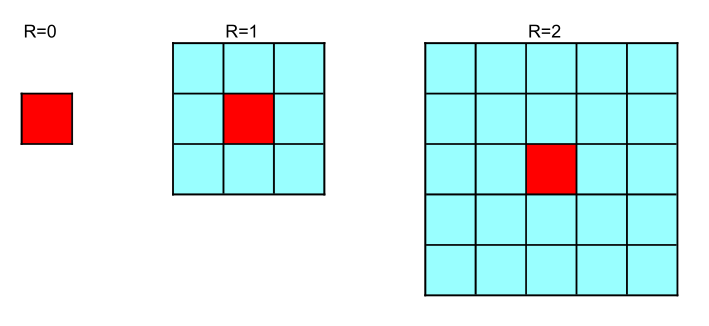
\includegraphics[scale=0.5]{moore.png} 
%\caption{Moore neighbourhood}
%\end{figure}
%\begin{figure}[H]
%\includegraphics[scale=0.5]{vonnewman.png} 
%\caption{VonNewman neighbourhood}
%\end{figure}
To not hardcode adding of neighbours to cell, following equations found in \cite{moore}\cite{vonnewman} were used:\\
\begin{equation}
	N^{M}_{x_0,y_0}=\{ \left(x,y\right): \mid x-x_0 \mid \leq r, \mid y-y_0 \mid \leq r   \}  
\end{equation}

\begin{equation}
	N^{V}_{x_0,y_0}=\{ \left(x,y\right): \mid x-x_0 \mid + \mid y-y_0 \mid \leq r   \} 
\end{equation}

\begin{itemize}
	\item $x_0,y_0$ - target cell coordinates
	\item $x,y$ - all other cells coordinates
	\item $r$ - neighbourhood size	
	\item $N^{V}_{x_0,y_0}$ - set of neighbours(VonNewman) cells for target cell
	\item $N^{M}_{x_0,y_0}$ - set of neighbours(Moore) cells for target cell
\end{itemize}

\subsection{Epidemic models}

SIR model was implemented with transition equations proposed by\cite{WHITE}. It was decided to use it, because :\\
\begin{itemize}
\item it takes vaccination into account
\item parameters of environment are considered
\item each cell has small population of individuals
\end{itemize}

\noindent SEIR model was implemented with transition equation proposed by\cite{cisse}.\\

\noindent SIS model was implemented, by changing SIR model equations.\\

%dodać listing kodu calculateNew state dla każdej klasy implementującej cell


\subsection{Code}
Program was written in Java. Simulation is created, by use of Timeline class, which object is used to execute doIteration() function. To avoid writing a lot of ifs and switches Factory pattern was used for creating Cell objects for chosen model.
%\begin{figure}[H]
%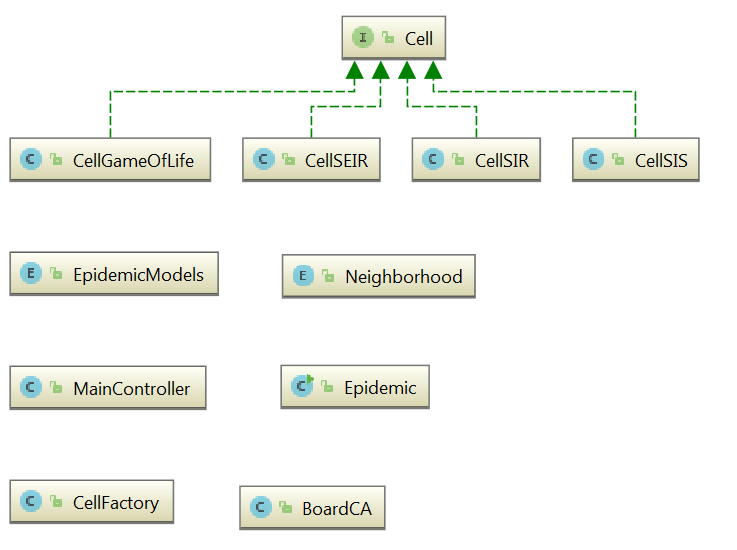
\includegraphics[width=\textwidth]{klasy.PNG} 
%\caption{Class diagram}
%\end{figure}
%\lstinputlisting{Cell.java}


For testing how code works and if program design is correct game of life was also implemented with not hard coded parameters.

\subsection{GUI}
The user interface was created with JavaFX and SceneBuilder.\\
%To start simulation:
%\begin{itemize}
%\item Choose model
%\item Choose neighbourhood type and size
%\item Set model parameters
%\item Click INIT button
%\item Change cell types, by mouse clicking(or dragging) on lattice (it is possible to choose new type of cell and cell parameters, depends on chosen model)
%\item Change speed of simulation on slider(optional, default 1s)
%\item To start click START button
%\item To pause click STOP button(you can resume with START button)
%\item Use CLEAR button to terminate simulation and be able to set up a new one

%\end{itemize}

\begin{figure}[H]
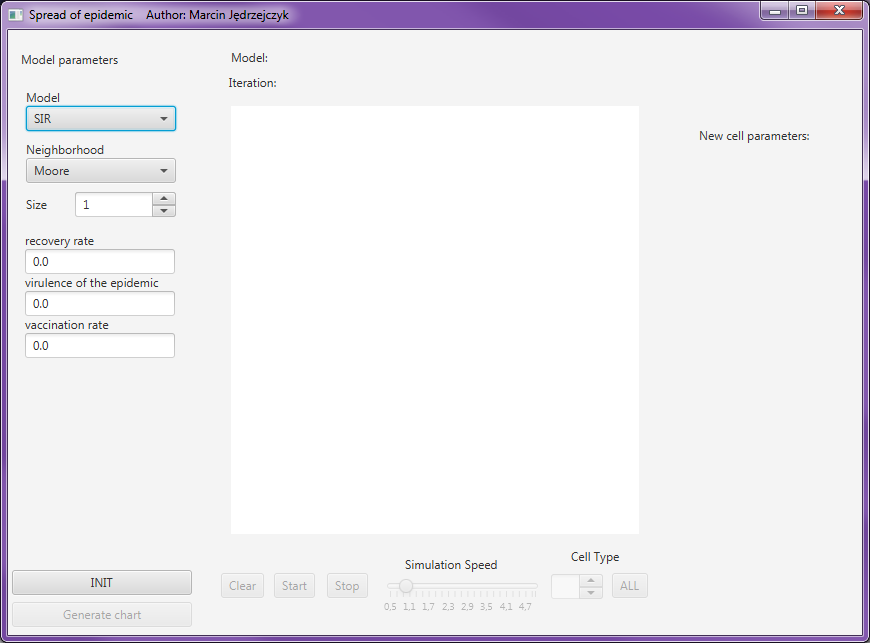
\includegraphics[width=\textwidth]{guiinit.PNG} 
\caption{GUI - program start}
\end{figure}
\iffalse
\begin{figure}[H]
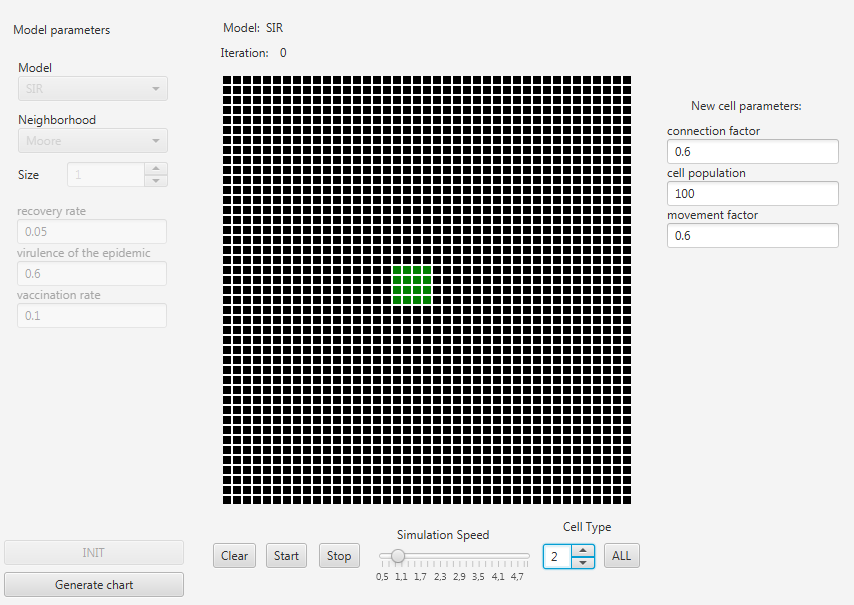
\includegraphics[width=\textwidth]{i0.PNG} 
\caption{GUI - simulation initialized(Iteration 0) }
\end{figure}
\begin{figure}[H]
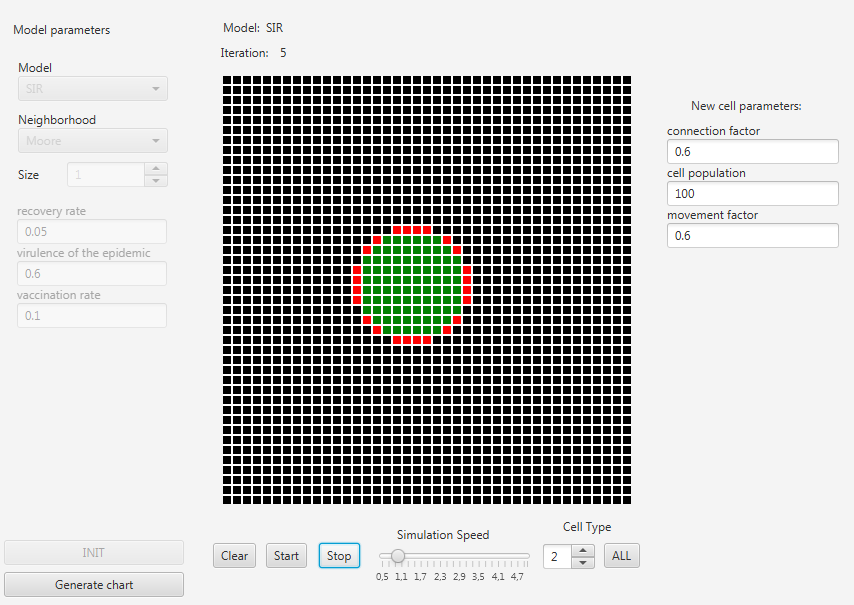
\includegraphics[width=\textwidth]{i5.PNG} 
\caption{GUI - Iteration 5}
\end{figure}
\begin{figure}[H]
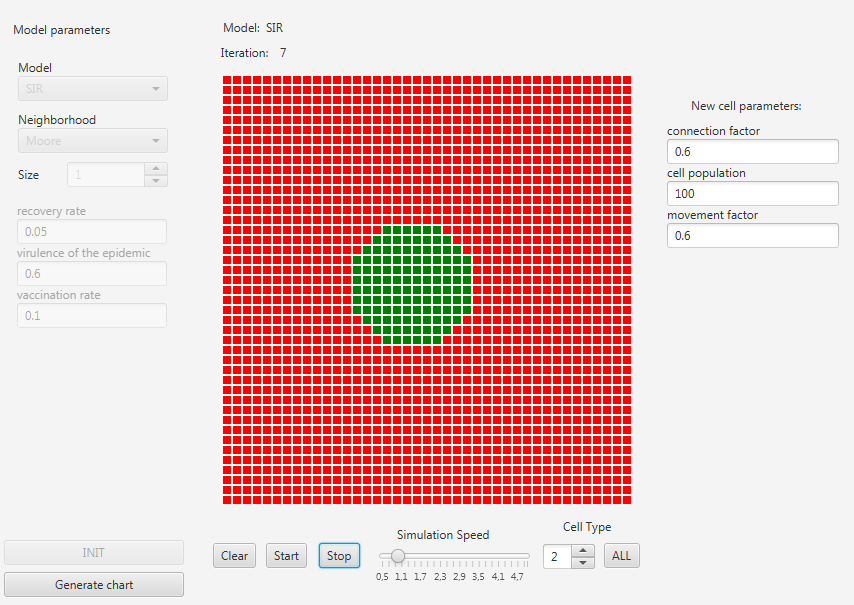
\includegraphics[width=\textwidth]{i7.PNG} 
\caption{GUI - Iteration 7}
\end{figure}
\begin{figure}[H]
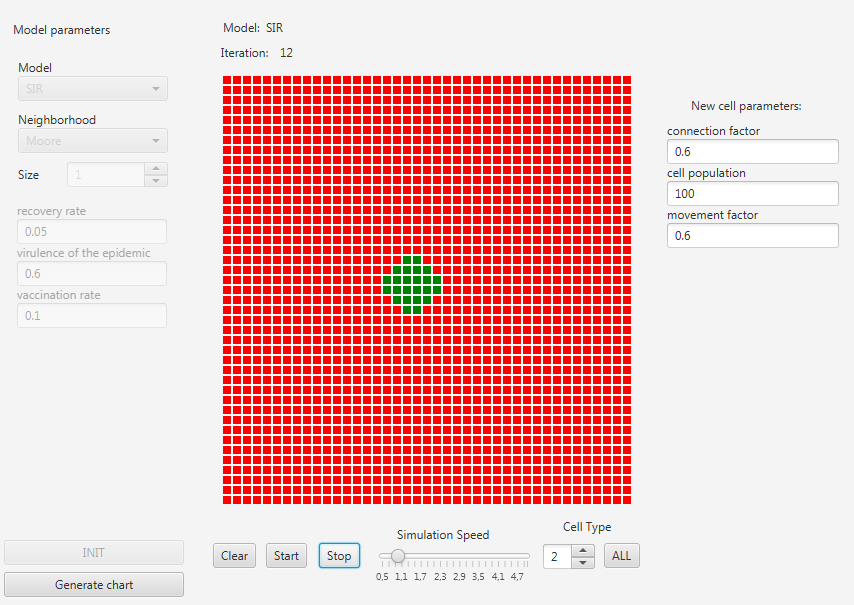
\includegraphics[width=\textwidth]{i12.PNG} 
\caption{GUI - Iteration 12}
\end{figure}
\fi
\section{Summary}
%TODO poprawki itp , lepsze entery wieksze przestrzenie
%The aim of this project is to implement SIR model of epidemic spread in cellular automata with JAVA. Main programming reference will be code from laboratory classes where cellular automata was used. The UI will be created with JavaFX and SceneBuilder. If possible interface  will have may parameters to choose, like: vaccination value,  people spread in lattice(random,uniform, constant), epidemic model(SIR,SIS,SEIR,SEIRS), neighbourhood size and type, if not only simple parameters for one model will be present.

The project main goal of implementing SIR model of the spreading of epidemics in Java was achieved. It was possible to also implement SEIR and SIS model. Testing program with game of life model proved that program design is acceptable.\\

Testing implementation of SIR model showed how great is impact of vaccination in preventing disease spreading. Also it possible to see quarantine, by use of empty cells or cells of recovery type(R). The following anomaly is observed when all cells have connection factor=1: instead of covering whole lattice with only 1 type of cells, program create symmetric symbol.\\

SEIR model is less precise when it comes to spreading disease from neighbours, because it only take into account Euclidean distance between cell and its neighbours and not like SIR model connection factor, movement factor and virulence of the epidemic.\\

It is advised to check more published papers to find better mathematical model for SIS model.\\

It is possible to add more models. Program was build with idea of addition of new models without big problems. It is proven, because implementation of SEIR model took less time than SIR model. What is more adding more parameters should not be a problem, because program stores them in hashmaps.
%TODO wnioski
%\bibliographystyle{plain}% plain/abbrv/alpha
%\bibliography{mybib}
\printbibliography

\end{document}
